\section{Methodology}
RegionCovOpt chooses one region per batch and evaluates one motion per trial (Fig.~\ref{fig:workflow}). A trial that improves the regional record immediately changes the archive. A later trial in the same batch can already use that point as its center. At the end of the batch, the selected trials guide the update of the regional distribution. The global incumbent determines where the next unreserved batch runs.

\begin{figure*}[t]\centering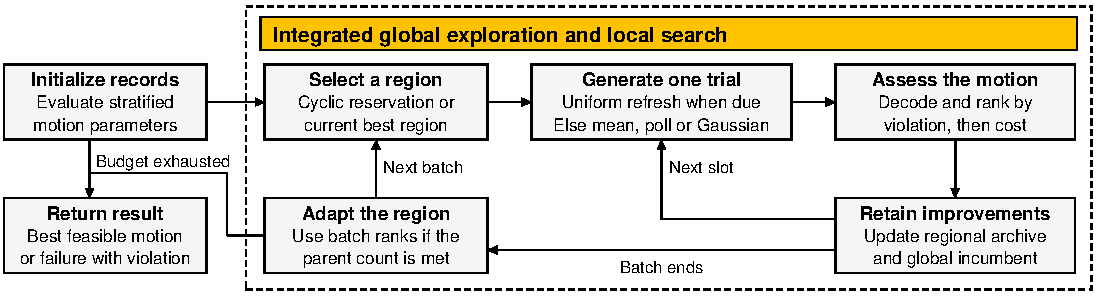
\includegraphics[width=.89\textwidth]{../figures/scheme.pdf}
\caption{Integrated search in RegionCovOpt. A reserved batch selects a region cyclically and includes one uniform refresh when its slot is reached. Other batches follow the global incumbent. Each trial updates the records on improvement. Batch ranks adapt the selected distribution when the parent count is met.}\label{fig:workflow}\end{figure*}

\subsection{Initialization and regional records}
The optimizer draws $N_0$ initial points by Latin hypercube sampling of the unit box. Its evaluation budget is $B$, and the number of regions is $K=|\mathcal I|$. The evaluator returns a decoded motion and its rank from Eq.~(\ref{eq:rank}). Each visited region stores its best record, including the least-violating candidate before the first feasible motion. Unvisited regions start with empty archives. The best record across all regions is the global incumbent.

Each region stores a mean $m_b$, covariance $C_b$, scale $\sigma_b$, and two evolution paths. An affine transformation maps the selector coordinate to the unit interval of the local search space. The other coordinates already use that scale. This gives relative perturbations the same meaning across regions of different widths. A region with $n_b$ initial points starts at the mean of its best $\min(q_0,n_b)$ points, where $q_0$ limits the initial parent count. An empty region starts at the box center. Each covariance starts at the identity, each path at zero, and each scale at $\sigma_0$.

\subsection{Allocation and trial generation}
Let $H$ denote the reservation period in batches. Every $H$th batch, starting with the first, visits the next region in cyclic order. Each intervening batch goes to the region of the current global incumbent. Before admission, the incumbent is the point with the least violation, with cost breaking ties. After admission it is the motion with the lowest feasible cost. Batch capacity and reservation period set the granularity and minimum revisit rate. The observed ranks determine which region receives the intervening batches, and the regional distribution determines the scale and direction of local steps.

Each batch has capacity $\lambda$. The mean slot evaluates the regional mean. The poll slot perturbs a uniformly chosen coordinate of the regional record by a centered Gaussian increment with standard deviation $\eta_0+\eta_1\sigma_b$ when that record exists. The refresh slot of a reserved batch draws a uniform point in local coordinates. The optimizer fills every remaining slot with a correlated Gaussian draw. Its center is the regional record for an archive-eligible slot in $\mathcal J_A$ with a record available, and the regional mean otherwise. Section~5 gives the slot order and parameter values.

For a covariance factorization $C_b=Q\Lambda Q^\mathsf{T}$ and center $c$, the Gaussian trial is
\Eq{trial}{y=c+\sigma_b Q\Lambda^{1/2}\varepsilon,\qquad \varepsilon\sim\mathcal N(0,I).}
The optimizer reflects each trial coordinate at the unit boundaries and maps it back to the selected region. Decoding and ranking the resulting motion counts as one evaluation. A better rank updates the corresponding records. Once an archive contains a feasible motion, its cost can only stay the same or decrease.

\subsection{Distribution update}
Order a completed batch by increasing lexicographic rank. Let $\mu$ be the number of selected parents, $y_{i:\ell}$ the $i$th ranked point among the $\ell$ evaluated trials and $w_i$ the normalized log weights. The optimizer also updates the distribution from a truncated final batch when $\ell\geq\mu$. In local coordinates, omitting the region subscript for readability,
\Eq{weights}{w_i=\frac{\log(\mu+1/2)-\log i}{\sum_{j=1}^{\mu}[\log(\mu+1/2)-\log j]},\qquad i=1,\ldots,\mu.}
\Eq{eff}{\mu_{\mathrm{eff}}=\left(\sum_{i=1}^{\mu}w_i^2\right)^{-1}.}
\Eq{mean}{m^+=\sum_{i=1}^{\mu} w_i y_{i:\ell}.}
Write $d_i=(y_{i:\ell}-m)/\sigma$ for a selected displacement and $d=(m^+-m)/\sigma$ for the mean displacement. The first path accumulates whitened mean displacements. The second accumulates mean displacements in regional coordinates.
\Eq{ps}{p_\sigma^+=(1-c_\sigma)p_\sigma+\sqrt{c_\sigma(2-c_\sigma)\mu_{\mathrm{eff}}}\,C^{-1/2}d.}
\Eq{pc}{p_c^+=(1-c_c)p_c+h\sqrt{c_c(2-c_c)\mu_{\mathrm{eff}}}\,d.}
The gate $h$ suppresses the addition to $p_c$ when the normalized step-size path exceeds the threshold. For region-local update count $t$, dimension $n$ and the reference Gaussian length $\chi_n$ defined in Appendix A,
\Eq{gate}{h=\mathbf{1}\!\left\{\frac{\|p_\sigma^+\|}{\sqrt{1-(1-c_\sigma)^{2t}}}<(1.4+2/(n+1))\chi_n\right\}.}
\Eq{factor}{\gamma=1-c_1-c_\mu+(1-h)c_1c_c(2-c_c).}
\Eq{cov}{C^+=\gamma C+c_1p_c^+(p_c^+)^\mathsf{T}+c_\mu\sum_{i=1}^{\mu} w_i d_i d_i^\mathsf{T}.}
\Eq{scale}{\sigma^+=\operatorname{clip}_{[\sigma_{\min},\,\sigma_{\max}]}\!\left(\sigma\exp\!\left[\frac{c_\sigma}{d_\sigma}\!\left(\frac{\|p_\sigma^+\|}{\chi_n}-1\right)\right]\right).}
Appendix A gives the learning rates from Hansen and Ostermeier~\cite{cma} and the eigenvalue floor for the factorization. A symmetric eigendecomposition requires $O(n^3)$ operations per batch. Sampling and covariance adaptation add $O(\lambda n^2)$ operations, in addition to the robot-dependent cost of the oracle.

Algorithm~\ref{alg:region} gives the slot and batch updates. Appendix B uses the independent refreshes to bound the probability of missing a positive-mass near-optimal set.

\begin{algorithm}[tbp]
\small
\caption{RegionCovOpt}\label{alg:region}
\KwIn{Scene, boundaries, maps $D$ and $R$, evaluation budget $B$, initial size $N_0$, regional proposal schedule, batch capacity $\lambda$, parent count $\mu$, reservation period $H$.}
\KwOut{Best admitted control and state histories and their terminal time, or failure.}
Evaluate the $N_0$ stratified points; initialize regional records, distributions and the global incumbent\;
\For{each batch $e$ while budget remains}{
  \eIf{batch $e$ is reserved}{select the next region in cyclic order\;}{select the region of the global incumbent\;}
  Factor the selected covariance; start an empty batch $\mathcal L$\;
  \For{each slot in the scheduled batch while budget remains}{
    \uIf{the slot is the mean slot}{set the trial to the regional mean\;}
    \uElseIf{it is the poll slot and a regional record exists}{perturb one coordinate of that record\;}
    \uElseIf{it is the refresh slot of a reserved batch}{draw uniformly in local coordinates\;}
    \Else{draw a correlated Gaussian about the record if the slot is archive-eligible and the record exists, or about the mean otherwise\;}
    Reflect and map to the selected region; decode the motion and evaluate its rank\;
    Append the trial to $\mathcal L$; update both records if improved\;
  }
  \If{$|\mathcal L|\geq\mu$}{
    Rank $\mathcal L$ and update the selected mean, evolution paths, covariance and scale using Eqs.~(\ref{eq:mean})--(\ref{eq:scale})\;
  }
}
\If{the global incumbent is admissible}{\KwRet{its control, state and terminal time}\;}
\KwRet{failure and the least violation found}\;
\end{algorithm}

